\begin{document}

The initial phase of creating the Application was to have a basic script which instantiates a Tensorflow model, processed the image to
Tensorflow standards and passed it on to the Model for object detection. Using this script as a basis which performed the object detection
on images,videos and web camera streams I started developing a application in Python with PyQt Version 5.\\
PyQt is a cross-platform GUI toolkit which is similar to Java Swift and is a easy library to develop a UI with, it takes ideas and concepts
from different roots and implements a layer based architecture for elements.
\begin{center}
    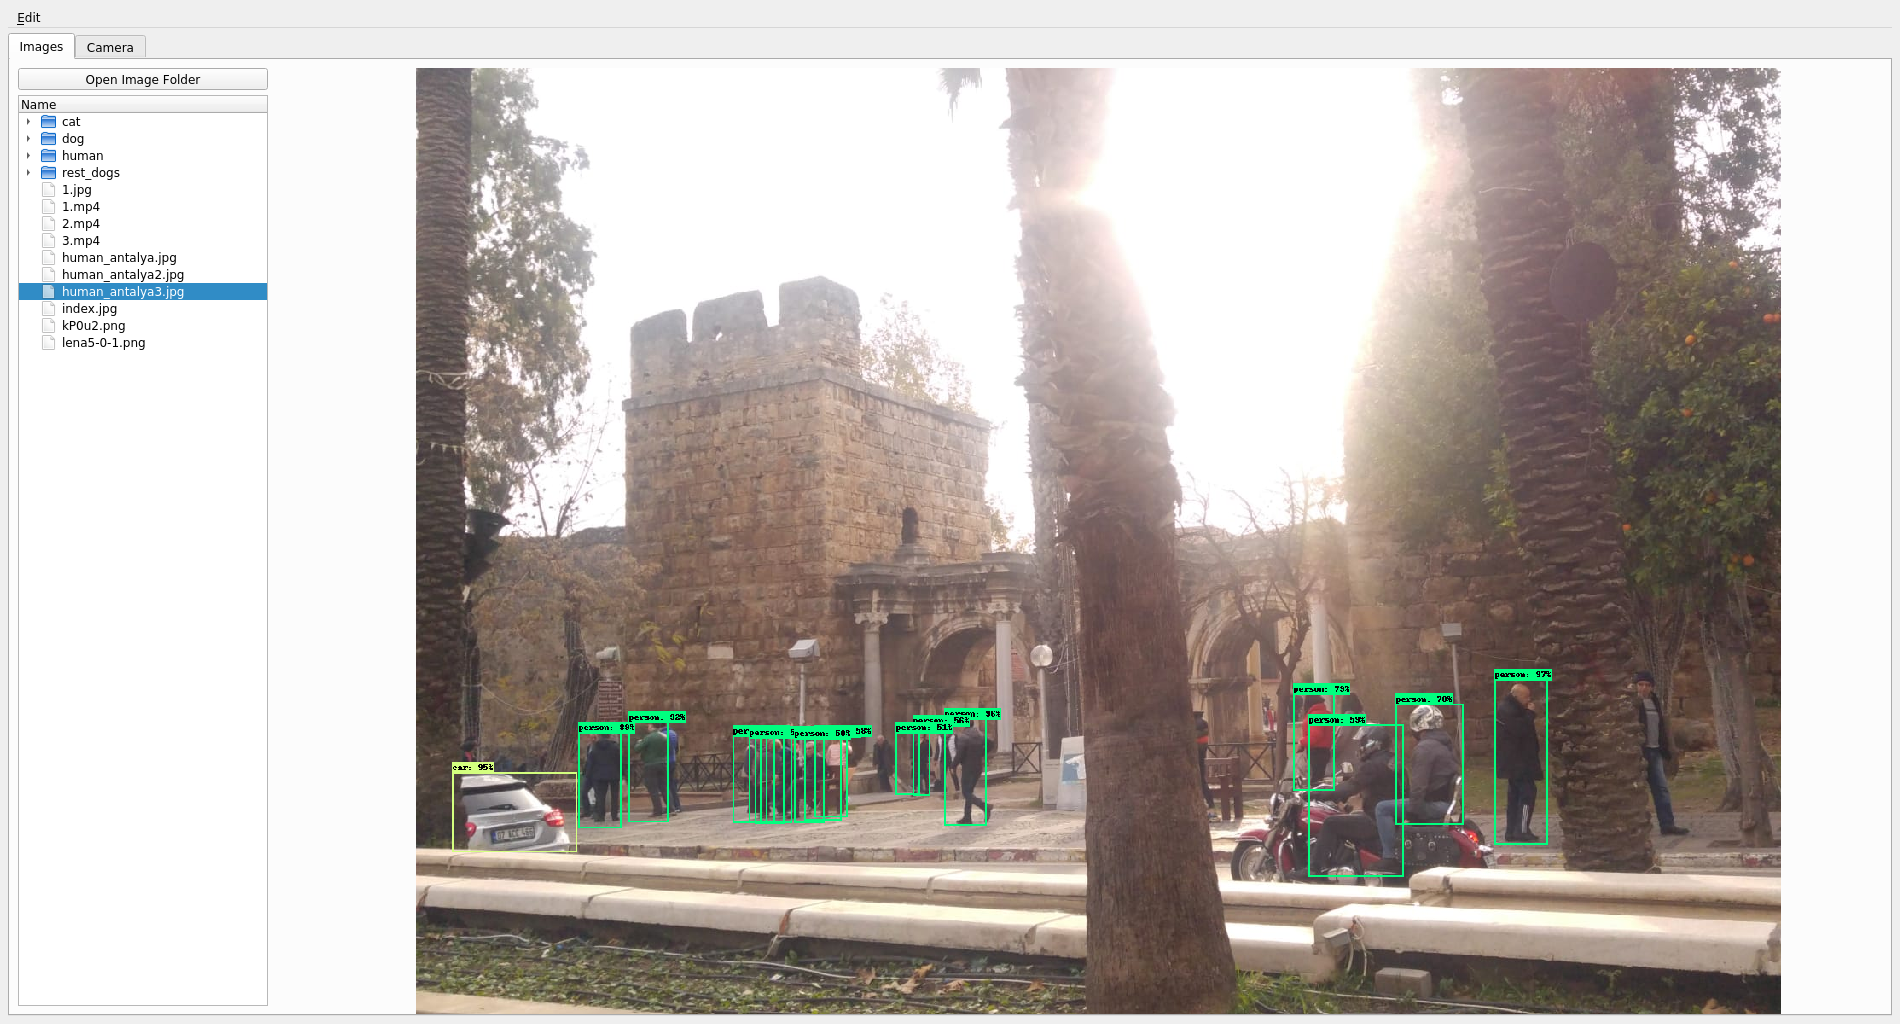
\includegraphics[width=0.75\textwidth]{images/application/Application.png}
\end{center}
There were several requirements for the Application from the start:
\begin{itemize}
    \item Use any model trained with Tensorflow \\ \\
        Since I am using the Tensorflos API for my application this point is being handled by Tensorflow itself
    \newpage \noindent
    \item Change used model, label map and class number on runtime \\ \\
        For this I implemented a config class where I will store the path's of the selected inference graph, the label map and the
        number of classes set by the User. These if existent will be queried for on startup and with them a Tensorflow model will be instantiated.\\
        \begin{center}
            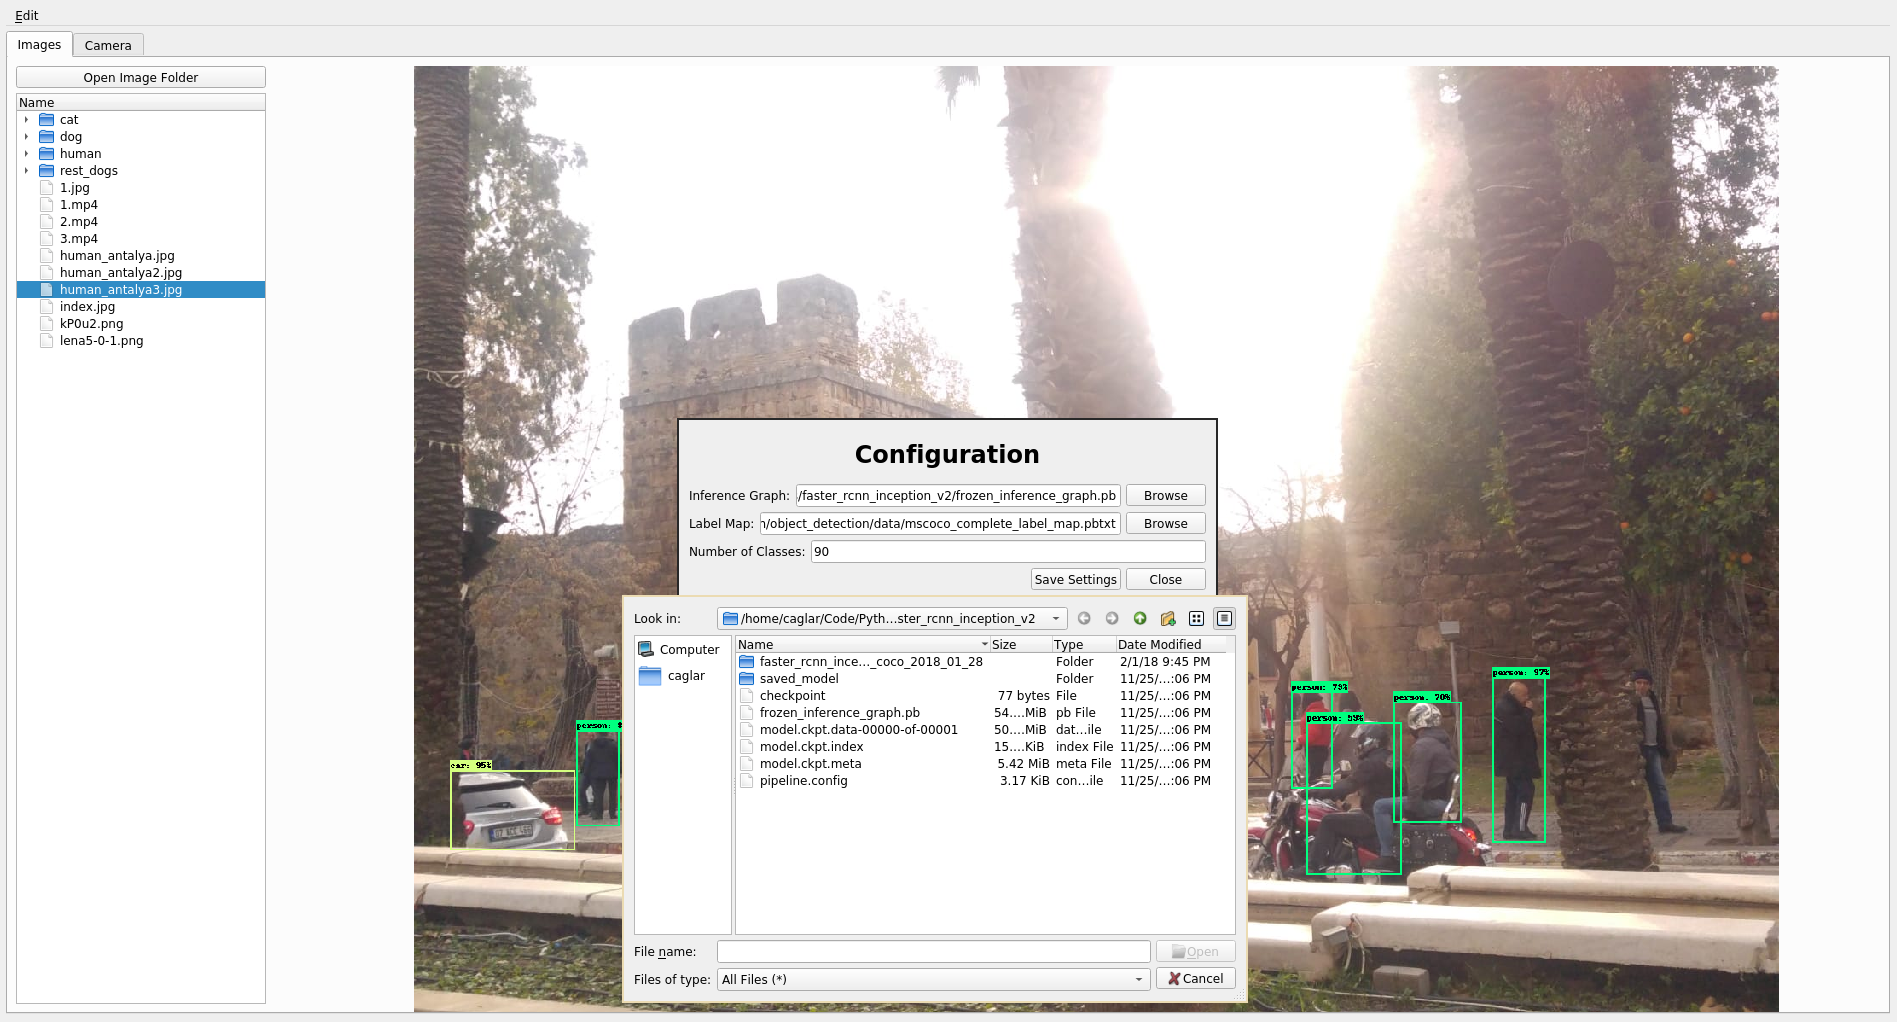
\includegraphics[width=0.75\textwidth]{images/application/application_config.png}
        \end{center}
    \item Initialize Tensorflow only when required (Application start, Configuration change)\\ \\
        To cover for the changes of the configuration I am checking if there are any changes in the configuration file and am recreating the
        Tensorflow Model on the Fly if not the old one will be used.
    \item Support Image, Video and Webcam detection \\ \\
        Once Tensorflow is instantiated the events of the application have to handled accordingly, with functionality implemented for each case.
        Since I went with the more explorer like feeling and implemented a TreeView as the source for the Files to select from a explorer
        was Implemented where you can select a folder as the root. Events and callback methods had to be written and passed over various
        classes to handle the selection of items, so an click is being interpreted as a object detection task. \\
        Images are being handled and rendered through PyQt however Video and Webcam streaming had to be implemented manually since PyQt had
        no option to access the data of the streams.\\
        To cover for this lack of functionality I used the package python-opencv and incorporated it into the work flow of PyQt. So Videos
        and Camera streams are analyzed frame by frame by opencv, converted then passed Tensorflow and finally converted back and displayed
        by PyQt.
\end{itemize} 

\end{document}
